%\documentclass[12pt,a4paper]{report}
\documentclass[12pt,a4paper,oneside,onecolumn,openright]{book}
% set the document language
\usepackage[italian]{babel}
% set the encoding used by your editor here (default is utf8)
\usepackage[utf8]{inputenc}
\usepackage[T1]{fontenc}

% math packages
\usepackage{amsmath}
\usepackage{amssymb}
\usepackage{lmodern}
% page margins settings
\usepackage[inner=3cm,outer=2.5cm,top=3cm,bottom=2.5cm]{geometry}
%\usepackage{indentfirst}

% other packages
\usepackage{array}
\usepackage{enumitem}
\usepackage{subfigure}
\usepackage{graphicx}
\usepackage{verbatim}
\usepackage{listings}
\usepackage{url}
\usepackage[hidelinks]{hyperref}
\usepackage[export]{adjustbox}
\usepackage{latexsym}
\usepackage{tabularx}
\usepackage{ragged2e}
\usepackage{mathtools}
\DeclarePairedDelimiter\floor{\lfloor}{\rfloor}
\DeclarePairedDelimiter\ceil{\lceil}{\rceil}
% \usepackage{Mathematics}
% custom colors
\usepackage{color}
\usepackage{wrapfig}
\usepackage{gensymb}
\usepackage{caption}
\usepackage{tikz}
\usepackage{forest}
\usepackage{tikz-qtree}

\newcommand\myeq{\stackrel{\mathclap{\tiny\mbox{def}}}{=}}

\usetikzlibrary{shadows}
\definecolor{light-gray}{gray}{0.96}
\definecolor{cyan}{RGB}{230,230,255}
\definecolor{dkgreen}{rgb}{0,0.6,0}
\definecolor{gray}{rgb}{0.5,0.5,0.5}
\definecolor{mauve}{rgb}{0.58,0,0.82}
\definecolor{iceberg}{rgb}{0.44, 0.65, 0.82}
% \definecolor{blue}{RGB}{44, 44, 210}

\hypersetup{
colorlinks=true,
linkcolor=black,
% filecolor=blue,
urlcolor=blue,
% pdftitle={Overleaf Example},
}

\urlstyle{same}
\graphicspath{ {./images/} }

% environment for bash code
\lstset{ %
  language=bash,                % the language of the code
  basicstyle=\footnotesize,           % the size of the fonts that are used for the code
  numbers=left,                   % where to put the line-numbers
  numberstyle=\footnotesize,          % the size of the fonts that are used for the line-numbers
  stepnumber=1,                   % the step between two line-numbers. If it's 1, each line 
                                  % will be numbered
  numbersep=5pt,                  % how far the line-numbers are from the code
  backgroundcolor=\color{white},      % choose the background color. You must add \usepackage{color}
  showspaces=false,               % show spaces adding particular underscores
  showstringspaces=false,         % underline spaces within strings
  showtabs=false,                 % show tabs within strings adding particular underscores
%  frame=single,                   % adds a frame around the code
  rulecolor=\color{black},        % if not set, the frame-color may be changed on line-breaks within not-black text (e.g. commens (green here))
  tabsize=2,                      % sets default tabsize to 2 spaces
  captionpos=b,                   % sets the caption-position to bottom
  breaklines=true,                % sets automatic line breaking
  breakatwhitespace=false,        % sets if automatic breaks should only happen at whitespace
  title=\lstname,                   % show the filename of files included with \lstinputlisting;
                                  % also try caption instead of title
  numberstyle=\tiny\color{gray},        % line number style
  keywordstyle=\textbf,          % keyword style
  commentstyle=\color{dkgreen},       % comment style
%  stringstyle=\color{mauve},         % string literal style
  escapeinside={\%*}{*)},            % if you want to add a comment within your code
  morekeywords={*,...,insert,-}               % if you want to add more keywords to the setù
}

% environment for python code
\lstset{
	language=Python,
	breaklines=true,
	breakatwhitespace=true ,
	backgroundcolor=\color{light-gray}
}

\newcommand{\grayScale}{0.95} % Can change the gray level here
\definecolor{codeBackground}{rgb}{\grayScale ,\grayScale ,\grayScale}
\definecolor{forestGreen}{rgb}{0.13,0.55,0.13}

\lstset{
    language=C,
    backgroundcolor=\color{codeBackground},
    tabsize=4,
    showstringspaces=false,
    showtabs=false,
    showspaces=false,
    basicstyle=\ttfamily,
    identifierstyle=\ttfamily,
    keywordstyle=\color{blue},
    stringstyle=\color{red},
    commentstyle=\color{gray},
    numberstyle=\color{magenta},
    morecomment=[l][\color{forestGreen}]{\#},
    escapechar={|}, 
}
% appendices package
%\usepackage{appendix}
% set Appendix name used in the toc
%\renewcommand{\appendixtocname}{Appendice}

% interline
\linespread{1.5}
% set numbers for subsections and show them in the toc
\setcounter{tocdepth}{3} 
\setcounter{secnumdepth}{3}

% layout package, style and settings
\usepackage{fancyhdr}
\pagestyle{fancy}

\fancypagestyle{mainmatter}{%		
		\fancyhf{} 
		\fancyhead{}
		\fancyhead[LE,RO]{\thepage}
		\fancyhead[LO]{\footnotesize{\leftmark}}
		\fancyhead[RE]{\footnotesize{\rightmark}}
		\fancyfoot{}
		\addtolength{\headwidth}{\marginparsep}
		\addtolength{\headheight}{2.5pt}
		\renewcommand{\headrulewidth}{0.3pt}
		\renewcommand{\footrulewidth}{0.0pt}
		}
\fancypagestyle{frontmatter}{%
		\fancyhf{} 
		\fancyhead[LE]{\footnotesize{\MakeUppercase{\thepage}}}
		\fancyhead[RO]{\footnotesize{\MakeUppercase{\thepage}}}
		\fancyhead[RE,LO]{}
		\fancyfoot{}
		\addtolength{\headwidth}{\marginparsep}
		\addtolength{\headheight}{2.5pt}
		\renewcommand{\headrulewidth}{0.0pt}
		\renewcommand{\footrulewidth}{0.0pt}
		}
		
		
\usepackage{fancyhdr}
\pagestyle{fancy}
		\fancyhf{} 
		\fancyhead{}
		\fancyhead[LE,RO]{\thepage} 
		\fancyhead[LO]{\footnotesize{\leftmark}}
		\fancyhead[RE]{\footnotesize{\rightmark}}
		\fancyfoot{}
		\addtolength{\headwidth}{\marginparsep}
		\addtolength{\headheight}{2.5pt}
		\renewcommand{\headrulewidth}{0.3pt}
		\renewcommand{\footrulewidth}{0.0pt}

% empty pages have no numbers
\makeatletter
\def\cleardoublepage{\clearpage\if@twoside \ifodd\c@page\else
\hbox{}
  %Potresti voler togliere il commento dalla linea seguente
  %Questa pagina � stata lasciata intenzionalmente vuota.
\thispagestyle{empty}
\newpage
\if@twocolumn\hbox{}\newpage\fi\fi\fi}
\makeatother
%????
%\textwidth=450pt\oddsidemargin=0pt

%\makeatletter 
%  \DeclareRobustCommand*\textsubscript[1]{% 
%    \@textsubscript{\selectfont#1}} 
%  \newcommand{\@textsubscript}[1]{% 
%    {\m@th\ensuremath{_{\mbox{\fontsize\sf@size\z@#1}}}}} 
\makeatother 

\begin{document}
\begin{titlepage}
\begin{center}
{
    \large
    \textbf{Università  degli studi di Modena e Reggio Emilia} \\
   	\textbf{Dipartimento di Ingegneria Enzo Ferrari} \\
    \vspace{\stretch{0.5}}
    \hspace*{0cm} \hrulefill \hspace*{0cm} \\
    \vspace{\stretch{0.5}}    
	  \vspace{\stretch{12}}
  
  
 		\huge{\bf Matematica Discreta }}\\
		\vspace{3mm}
		
		\vspace{\stretch{6}}
		\end{center}
		
\vspace{40mm}
\par
\noindent
\vspace{20mm}
\begin{center}
\hspace*{0cm} \hrulefill \hspace*{0cm} \\
{\large{\bf 
Anno Accademico 2023/24}}
\end{center}

\end{titlepage}

\pagestyle{frontmatter}
\frontmatter

% PAGINA VUOTA
%\clearpage\null\thispagestyle{empty}\clearpage
\setcounter{tocdepth}{2}
\tableofcontents

\setlength{\parindent}{12pt}
\setlength{\parskip}{1ex plus 0.5ex minus 0.2ex}
\mainmatter
\pagestyle{mainmatter}

\chapter{Introduction}

\section{Structure and Content}
\begin{itemize}

    \item \textbf{Module 1}: 
    \begin{enumerate}
        \item \textbf{\textit{intra-vehicles communications}}: nodes, sensors, ECU
        \item \textbf{\textit{signal busses}}: CAN, LIN, FlexRay, MOST, Ethernet [ T1/T1S]
        \item \textbf{\textit{car domain and OS}}
    \end{enumerate}
    
    \item \textbf{Module 2}:
    \begin{enumerate}
        \item \textbf{\textit{inter-vehicles communications}}: \textit{V2V} and \textit{V2X} (car is a node)
        \item \textbf{\textit{wireless technologies}}: Bluetooth, LoRa, C-V2X, IEE 802.11p (bd)
        \item application, messages, broadcast, GPS
    \end{enumerate}

\end{itemize}
Different \textbf{domain} or \textbf{application} needs different \textit{communications protocols}, is important to understand how each nodes in domain communicate each other (inside the car).

\newpage
\section{Intra-Vehicles}
From the 80's, where the car's control unit are isolated an there was a dedicated wires connect sensors and actuators with less electronic than now, until the reach the greates goal of evolution in the automotive sector: autonomous drive. The complexity of the number of connection from each ECU's to the other, also the number of ECU's for each car, is growing. While the number of signal increase in a liner way, the connection between ECU's is growing with a quadratic complexity $O(n^2)$.

If we examine the evolutions of the ECUs number inside an ``Audi A6'' we can observe that in 1997 it has 5 ECUs and in the 2007 it has 50 ECUs, instead the ``Tesla M3'' in the 2017 has 70 ECUs. The quadratic increase of ECUs number, however has reach a cap for two main reason: the cost and the space inside the car. Traditionally one ECUs is responsible of one task, but nowadays it could be two type of trends:
\begin{enumerate}[nosep]
    \item \textit{distributed of function across ECUs}
    \item \textit{integration of multiple function in one ECU}
\end{enumerate}

\section{Architectures}

\begin{figure}[h]
    \centering
    \begin{minipage}[t]{0.45\textwidth}
        \centering
        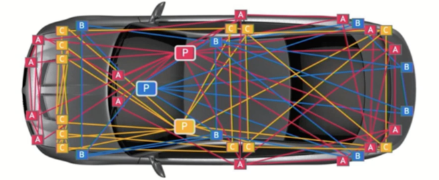
\includegraphics[width=\textwidth]{img/domain_architecture}
        \caption{\textit{Domain Architecture}}
        
        \begin{flushleft}
            \begin{enumerate}[nosep]
                \item central domain controller (\textbf{P}) or high performance computer
                \item ability to handle more complex functions
                \item cost optimization
                \item cable harness is rigid and expensive
            \end{enumerate}
        \end{flushleft}

    \end{minipage}
    \begin{minipage}[t]{0.45\textwidth}
        \centering
        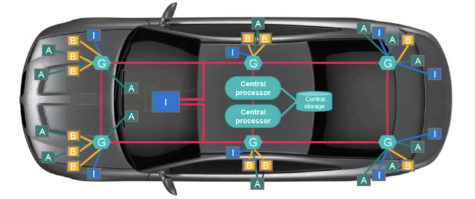
\includegraphics[width=\textwidth]{img/zonal_architecture}
        \caption{\textit{Zonal Architecture}}
        
        \begin{flushleft}
            \begin{enumerate}[nosep]
                \item local ethernet per zone (\textbf{G})
                \item ultra high-speed secured backbone between zone
                \item centralized software
                \item central computer storage
            \end{enumerate}
        \end{flushleft}
        
    \end{minipage}
\end{figure}
\chapter{Parte 3}
\section{Strutture algebriche elementari}
Una \textbf{operazione binaria intera} su un insieme G è un'applicazione 
\begin{center}
    $\ast \; : \; G \times G \rightarrow G$
\end{center}
L'immagine della coppia $(x,y)$ si denoterà con $x \ast y$. 
\begin{itemize}
    \item $e \in G$ si dice \textbf{elemento neutro} rispetto a $\ast$ se:
    \begin{center}
        $g \ast e = e \ast g = g \; \forall g \in G$
    \end{center}
    \item un elemento $g \in G$ si dice invertibile se esiste $\bar{g} \in G$ tale che $g * \bar{g} = \bar{g} * g = e$
\end{itemize}

\subsection{Gruppi}
La coppia $(G, \ast)$, con $\ast$ operazione su G, si dice \textbf{gruppo} se vengono rispettate le seguenti proprietà:
\begin{itemize}
    \item $\ast$ è \textbf{associativa}: $\forall g, g', g'' \in G$ si ha $(g \ast g') \ast g'' = g \ast (g' \ast g'')$
    \item esiste l'elemento \textbf{neutro}
    \item ogni elemento di G è invertibile
\end{itemize}
Il gruppo si dice \textbf{abeliano} o \textbf{commutativo} se: 
\begin{center}
    $\forall g, g' \in G, \; g \ast g' = g' \ast g$ (proprietà \textbf{commutativa})
\end{center}
Alcuni \textcolor{yellow}{\textbf{esempi}}:
\begin{itemize}
    \item $(\mathbb{N}, +)$, $(\mathbb{Z}, \cdot)$ non sono gruppi. in quanto non né in $\mathbb{N}$ e $\mathbb{Z}$ sono presenti per ogni elemento dell'insieme dell'elemento inverso, in $\mathbb{N}$ non sono presenti elementi negativi, quindi nessun elemento avrà un'altro che sommato a se stesso dia 0, viceversa l'insieme $\mathbb{Z}$ che sono presenti elementi positivi e negativi viene definita l'operazione $\cdot$ richiede i reciproci dei singoli elementi affiché possano essere definiti gli elementi inversi.
    \item $(\mathbb{Z}, +)$, $(\mathbb{Q}, \cdot)$ sono gruppi abelliani
\end{itemize}

\subsection{Anelli}
La terna $(\mathbb{A}, +, \cdot)$ con $\mathbb{A}$ un insieme e $+, \cdot$ (somma e prodotto) due operazione binarie interne a $\mathbb{A}$, si dice \textbf{anello} se:
\begin{itemize}
    \item $(\mathbb{A}, +, \cdot)$ è un gruppo \textbf{abeliano} (con elemento neutro 0).
    \item il prodotto è \textbf{associativo}.
    \item per ogni $x,y,z \in \mathbb{K}$ si ha $x \cdot (y + z) = (x \cdot y) + (x \cdot z)$ e $(x + y) \cdot z = (x \cdot z) + (y \cdot z)$ (il prodotto è distribuito rispetto alla somma).
\end{itemize}
Un anello $(\mathbb{A}, +, \cdot)$ è detto \textbf{commutativa} se il prodotto è commutativo, mentre è detto \textbf{unitario} o con \textbf{unità} se $(\mathbb{A}, \cdot)$ ammette l'elemento neutro. $(\mathbb{Z}, +, \cdot)$, $(\mathbb{Q}, +, \cdot)$, $(\mathbb{R}, +, \cdot)$, $(\mathbb{C}, +, \cdot)$ sono anelli.

\newpage
\subsection{Campi}
La terna $(\mathbb{K}, +, \cdot)$ con $\mathbb{K}$ un insieme e $+, \cdot$ (somma e prodotto) due operazioni binarie interne a $\mathbb{K}$, si dice \textbf{campo} se:
\begin{itemize}
    \item $(\mathbb{K}, +)$ è un gruppo \textbf{abeliano} (con elemento neutro 0).
    \item $(\mathbb{K} - \{0\}, \cdot)$ è un gruppo \textbf{abeliano} (con elemento neutro 1).
    \item per ogni $x,y,z \in \mathbb{K}$ si ha $x \cdot (y + z) = (x \cdot y) + (x \cdot z)$ quindi il prodotto è distribuito rispetto alla somma.
\end{itemize}
In qualunque campo vale la \textbf{legge di annullamento del prodotto}:
\begin{center}
    $x \cdot y = 0 \rightarrow x = 0 \; \text{oppure} \; y = 0$
\end{center}

\subsection{Domini d'integrità}
\textbf{Divisori dello zero}: sia $(A, +, \cdot)$ un anello. Due elementi $a,b \in A$ si dicono \textbf{divisori dello zero} se $a \neq 0$, $b \neq 0$, ma $a \cdot b = 0$. Ad \textcolor{yellow}{\textbf{esempio}} l'anello delle matrici quadrate presenta dei divisori dello zero. \\
Un anello commutativo privo di divisori dello zero si dice \textbf{dominio di integrità}, ad \textcolor{yellow}{\textbf{esempio}} $(\mathbb{Z}, +, \cdot)$ è un anello commutativo unitario privo di divisori dello zero. Quindi è dominio di integrità.

\section{L'anello dei numeri interi}
È noto che $\exists h \; | \; h : \mathbb{Z} \rightarrow \frac{\mathbb{N}_0 \times \mathbb{N}_0}{\mathcal{R}}$ dove la relazione di equivalenza che si vuole definire è $\equiv_n$. Su questo insieme vengono \textbf{ben poste} le seguenti operazioni:
\begin{center}
    $\boxplus : \mathbb{Z} \times \mathbb{Z} \rightarrow \mathbb{Z}$ \\
    $((m, n), (m', n')) \mapsto [(m, n)] \boxplus [(m', n')] \myeq [(m + m', n + n')]$

    $\boxdot : \mathbb{Z} \times \mathbb{Z} \rightarrow \mathbb{Z}$ \\
    $((m, n), (m', n')) \mapsto [(m, n)] \boxdot [(m', n')] \myeq [(mm' + nn', mn' + m'n)]$
\end{center}
Definito questo possiamo dire che $(\mathbb{Z}, \boxplus, \boxdot)$ è \textbf{dominio di integrità}.

\section{Teoria della Divisibilità}
\textbf{Divisibilità}: dati due numeri $a,b \in \mathbb{Z}$, si dice che $a$ \textbf{divide} $b$ (e si scrive $a|b$) se:
\begin{center}
    $\exists c \in \mathbb{Z} \; | \; b = a \cdot c$
\end{center}
\textbf{Transitività}: se $n|m$ e $m|q$ allora $n|q$. \\
\textcolor{green}{\textbf{Dimostrazione}}: per ipotesi $\exists h \in \mathbb{Z} \; | \; m = h \cdot n$ e $\exists h' \in \mathbb{Z} \; | \; q = h' \cdot m$. Sostituendo la prima relazione nella seconda si ottiene $q = h' \cdot h \cdot n$. Poichè $h' \cdot h \in \mathbb{Z}$ abbiamo definito che $n|q$. \\ \newline
Se $n|m$ e $m|n$, allora $m \pm n$. \\
\textcolor{green}{\textbf{Dimostrazione}}: per ipotesi $\exists h \in \mathbb{Z} \; | \; m = h \cdot n$ e $\exists h' \in \mathbb{Z} \; | \; n = h' \cdot m$ andiamo a sostituire la seconda alla prima equazione:
\begin{center}
    \begin{align*}
        n &= h' \cdot h \cdot m \\
        n - h' \cdot h \cdot m &= 0 \\
        n \cdot (1 - h' \cdot h) &= 0
    \end{align*}
\end{center}
Essendo che $\mathbb{Z}$ è un \textbf{dominio di integrità}, segue che o $n = 0$ oppure $(1 - h' \cdot h) = 0 \rightarrow (h' \cdot h) = 1$, consideriamo che $n \leq 0$ e che quindi $h' \cdot h = 1$ sappiamo che $h$ ammette un inverso $h'$, da cui $h = h' = 1$ o $h = h' = -1$ (in $\mathbb{Z}$, gli unici elementi che ammettono inverso sono $1$ e $-1$). In questo modo sappiamo che $m=n$ oppure $m=-n$.

\section{Massimo Comune Divisore}
Dati $a,b \in \mathbb{Z}$ non entrambi nulli, si dice che $d \in \mathbb{Z}$ è \textbf{UN massimo comune divisore} tra $a$ e $b$ se:
\begin{itemize}
    \item $d|a$ e $d|b$
    \item $\forall d' \in \mathbb{Z} \; | \; d'|a, \; d'|b \Rightarrow d'|d$
\end{itemize}
Se $d$ e $d'$ sono due massimi comuni divisori tra $a$ e $b$ allora $d' = \pm d$.


% PAGINA VUOTA
%\clearpage\null\thispagestyle{empty}\clearpage
%\appendix
%\appendixpage
%\addappheadtotoc

%\clearpage\null\thispagestyle{empty}\clearpage


%\listoffigures


\begin{flushleft}
\bibliographystyle{plain}
\bibliography{sections/references} 
\end{flushleft}

\end{document}
